\chapter{Problem analysis}
We divide the analysis into three steps.
In the first section, we think of potential users of the integration in order to define realistic use cases for them.
Four use cases describe the user's intentions.
Then, we specify requirements, which are demanded by the use cases.
In the last section, we propose a high-level architecture of our solution, where we aim at utilizing Blazor and Peachpie to cover the requirements.

\section{Use Cases}
We remind technologies of interest to introduce a context of our use cases.
PHP is used for server scripting, where it is designed to process a request, create the website, and send it back.
Blazor is a web framework for creating a client-side UI using C\#.
Peachpie is a PHP compiler, which compiles a collection of PHP scripts, representing a standalone project, to a .NET assembly.
\par
A user persona \squarecite{27} is a description of an imaginary user, which represents the needs of some group of users.
We use four user personas to cover use cases, which help us to identify requirements.
\par
The first persona is a C\# programmer, Blake, excited for Blazor.
He has already got acquainted with our solution.
\par
The second persona is a PHP programmer, Alice, who has no experience with Blazor but knows Peachpie basics.
Alice creates standard websites written in PHP, where she uses techniques introduces in the PHP section.
One day Blake tells her about our solution to migrate the scripts to a browser using Blazor and Peachpie.
She is excited by the solution and looks forward to using it.
However, she does not want to learn the Blazor framework.
\par
The third persona is a PHP programmer, Bob, who has already tried to write a simple website using Blazor and knows Peachpie basics.
He creates standard PHP websites similar to Alice's.
One day Blake tells him about our solution, and Bob's wish is to use the solution to help him inject his PHP scripts into Blazor websites.
Occasional work with the Blazor framework does not bother him, but it should have appropriate difficulty to his skills.
\par
The fourth persona is an enthusiastic PHP programmer, Chuck, who has advanced experience with Blazor and knows Peachpie basics.
He does not avoid exploring new technology to utilize all their aspects.
Blake tells him about our solution, and Chuck wishes that the solution offers him to collaborate with Blazor by PHP.
\par
These descriptions should help us determine the following use cases, which are realistic to them.
We call the first use case \textbf{Web} aiming at Alice.
We suppose she has a simple PHP website, which contains some information about her company.
The website does not work with a database and consists of pages containing images and references interconnecting them.
Some pages are adjustable by specifying the query part of the URL, and they include other scripts to add some basic layout.
One day the website notices many accesses, and Alice wants to migrate the website in order to a client side to save server resources.
The migration should download most of the website to a browser.
Afterward, navigation between scripts and script execution should be maintained on the client side.
Even more, Alice does not want to adjust the website for a client side too much, and she wishes for a simple solution that is understandable by a novice.
\par
We call the second use case \textbf{OneScript} aiming at Bob, who already has some experience with Blazor.
He wants to contribute to an existing Blazor website.
He has a great idea of adding a new widget, displaying the user's graph using HTML and CSS.
Because he is used to PHP, he wants to implement it with a few PHP scripts, which use some supporting libraries.
The idea consists of letting the user choose to load graph data from a file or generate a predefined graph as a demo.
After that, the widget renders HTML markup representing the graph.
Bob uses forms to interact with a user, and he is not willing to learn Javascript or interoperability between PHP and Blazor.
Thus, he needs a solution, which offers interaction with a user and uses standard PHP conventions mentioned earlier.
\par
We call the third use case \textbf{WebGame} aiming at Chuck.
He wants to create a real-time web game similar to Asteroids written in PHP.
He decides to target on a client side and utilizes Blazor, Peachpie, and our solution.
A client side execution should prevent network latency by loading the game in the beginning.
After that, the game will be independent of the network connection due to running the game and saving the game state by a browser.
PHP programmers have not been used to saving variables or defined functions across scripts because of the HTTP policy mentioned in the PHP section.
However, Chuck utilizes state persistent to saves a state of all game entities in variables.
Because he has previous experience with Blazor infrastructure, he will appreciate utilizing all Blazor aspects to run this game.
\par
\begin{figure}[t]\centering
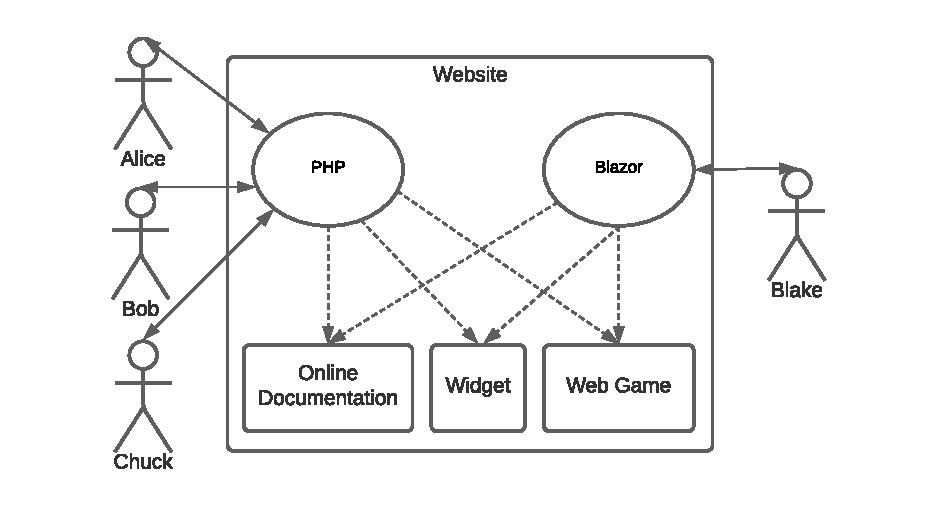
\includegraphics[scale=0.8]{./img/UseCaseAllTogether}
\caption{The AllTogether use case describing the combination of the all previous use cases. Double-headed arrows represent the person's used language. Dashed arrows represent a possible usage, where the head aims to an implementation written in the language.}
\label{img09:usecase}
\end{figure} 
\par
We can see an illustration of the fourth use case, which we call \textbf{AllTogether}, in Figure \ref{img09:usecase}.
The goal of the use case is to allow collaboration between PHP and Blazor programmers, where a difference of languages is not a barrier.  
We can image two teams creating a web application. 
They agreed on developing a client-side web application, where both teams aim at different parts of the website.
For example, one team wants to create a fun zone where a user can play some web game, we can imagine something like Asteroids, and the second team wants to create some online documentation about the game and the widget for the graph representation displaying a user's score.
Because Blazor targets client-side web applications, they want to utilize Blazor.
Unfortunately, these teams use a different favorite language, where the first team uses PHP and the second team uses C\#.
Even more, these teams want to contribute to any part of the Blazor website, meaning that doing the fun zone can be handled by either the C\# or PHP team.
They need some environment where the PHP team can code alongside the Blazor team, and they can focus on an arbitrary part of the web application.
We can see the intention in Figure \ref{img09:usecase} where each team can create a part aiming at the web game, the online documentation, and widget.
We can see the PHP team consists of Alice, Bob, and Chuck, having different skills with Blazor, so the environment should reflect it.
Even more, Blake should be able to manipulate their part of the application to customize it using C\#. For example, he should change the layout of the website without complex refactoring. 

\section{Requirements}

The goal of this section is to describe requirements based on mentioned use cases.
If the proposed solution covers the requirements, then PHP scripts will become a valuable part of a Blazor website.
\par
\textbf{Navigation} is the first requirement that our solution should provide.
We demonstrate navigation posibilities in Figure \ref{img10:scripts}.
Basic functionality should provide script routing, which finds a script by its name, executes it, and displays the output in a browser.
The solution should offer a straightforward router making a PHP website accessible, as we can see in the figure.
The simplicity is a necessary condition for the \textit{Web} use case and should be reflected.
Blazor should navigate components defined in \texttt{script.php} due to the \textit{WebGame} use case, which uses Blazor structures.
\par
\textbf{Reusability} of script is an important feature to make the \textit{OneScript} use case more useful.
Thus, Bob can insert the widget in different parts of the website, meaning that he can create a new web page containing some content and insert the widget into it, as we can see in Figure \ref{img10:scripts} where the Blazor component is generated from a PHP script and a Razor file.
\par
\begin{figure}[t]\centering
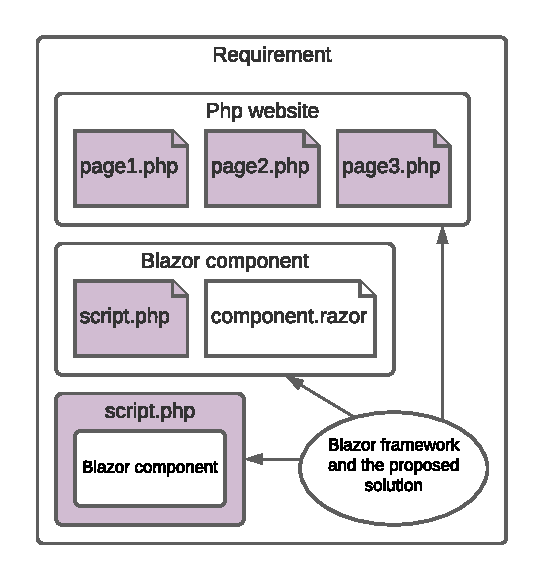
\includegraphics{./img/Requirement}
\caption{The requirement describing navigation between different types of entities. 
The first one represents a collection of script routable by default \texttt{Router}.
The second represents a standard component contenting a PHP code, and the last contains a defined Blazor component in the script.
The proposed solution with Blazor connects these types into a single website, where they can live together.
}
\label{img10:scripts}
\end{figure} 
\par
\textbf{Interactivity} with a user is necessary in the \textit{WebGame}, and \textit{OneScript} use cases.
The solution should enable using common conventions in PHP, like forms, and be able to utilize Blazor features providing the interaction as well.
\par
\textbf{Rendering} should be maintained in two ways.
The first way aims at the \textit{Web} use case when a script output is transparently displayed as a web page or its fragment.
The approach hides Blazor infrastructure for rendering a markup and makes creating a UI easier for PHP programmers.
The second way aims at the \textit{WebGame} use case when the solution provides an interface for the interaction with Blazor.
It is also necessary when we want to use already defined components in a PHP code.
The rendering should be effective due to the high frame rate of the game.
\par
\textbf{State preservation} should be available for creating a web application by a collection of scripts saving their variables after the execution.
This feature is not typical for PHP because of PHP policy and conventions, where programmers are used to deletion of variables and function definitions after the request termination.
The state described by the variables needs to be preserved in order to interact with a user in a client-side application. 
For an example, the \textit{WebGame} use case uses variables to save the game state. 
However, we have to distinguish these situations where the feature is necessary.
\par
\textbf{Server simulation} should be the main advantage of the solution.
We could see superglobals are commonly used methods how to obtain information about navigation or submitted data.
The solution should support superglobals for examples like the \textit{Web} use case, where the website uses information about URL query part, via \texttt{\$\_GET} variable, to make decisions.
\par
\textbf{Forms} should be maintained by the solution. 
The forms are usually sent to a server, but the solution should handle them on a client side, where they should be provided to PHP scripts.
After navigation to a script defined in the \texttt{action} attribute, the script should access the form data.
We can upload files by form.
Thus, the solution should provide file management accessing and downloading them.
\par
\textbf{Interoperability} between PHP, Blazor, and Javascript should be supported for situations when forms, the server abstraction, or Blazor are not sufficient.
We need some representation of Blazor in PHP, which the \textit{WebGame} use case will use for interacting with a Blazor.
Javascript is essential for client side applications, and we should be able to use its features.

\section{Architecture}

The basic principle of our solution consists of PHP scripts compilation into .NET assembly by Peachpie.
After that, a Blazor App references \texttt{Peachpie.Blazor}, which is a support library providing a mechanism for navigating and executing the scripts.
Then, a server provides the application to a browser, where Mono runtime executes it.
We will describe the architecture from the view point of compilation time and runtime.
\par
When we think about PHP script compilation, there are two possibilities.
We can compile the scripts ahead of time and reference them from a Blazor App. 
The second way is to regard the scripts as Static Web Assets and load them into a browser as separated files.
Afterward, the Peachpie compiles and executes them.
Both approaches have different advantages. 
Thus, there is no silver bullet.
The first approach saves time by ahead compilation and compilation check.
However, the second approach can save browser memory when the web application is larger, and a client uses only a part of it.
We are inclined to the first approach because the static compilation is a standard way in Peachie.
We think that the first approach is valuable for the use cases mentioned earlier.
The \textit{Web} use case wants to save additional requests. 
The rest of the use cases intends to utilize small amounts of PHP scripts as a part of the website, so we suppose that the smaller size of resulting scripts is insignificant in contrast with the compiled Peachpie assembly, containing all of them. 
\par
We have to figure out how to attach a PHP code, which is compiled into the assembly, to the Blazor App.
Although Peachpie supports calling functions written in PHP from Blazor by default, we want to create an abstraction over the Blazor environment in order to simplify the interface.
The abstraction should offer a representation of PHP scripts in Blazor.
It should allow an option for accessing the Blazor interface for advanced features.
It should be compatible with the Blazor environment in other to allowing a smooth collaboration between the abstraction and the Blazor pages.
A Blazor page consists of components, which can collaborate with each other.
Thus, we can utilize them to represent PHP scripts.
Components can be arbitrarily put together, which offers to place our PHP code in the desired place in the Razor code.
Even more, we can replace a root component, \texttt{Router} by default, with the component representing PHP scripts.
Afterward, scripts will compose the whole Blazor website content.
The component provides a sufficient Blazor interface for rendering control and interaction with a browser. 
\par
We can think about how to represent PHP scripts as components.
We can consider one type of component, which will provide the abstraction for all the PHP code in scenarios.
A problem with this approach is that the use cases need different levels of abstraction.
The \textit{WebGame} use case wants to use the component for offering the Blazor interface accessible from PHP code.
The offer should contain identical or similar options, which are given in a C\# code.
The \textit{OneScript} use case wants to free a programmer from Blazor.
Thus, we want to use the component as an adjustable provider finding and executing PHP scripts.
Its purpose is to keep the user away from knowing about the detailed structure of Blazor and the integration.
Another important thing is a provider role in a Blazor App.
The provider can behave either as default Blazor \texttt{Router} or as a routable component, which enables the navigation of PHP scripts.
As a consequence, we need to create more types of components providing abstractions for the particular use cases.
However, only one type of component can manage all provider roles due to their similar rendering transparency.
The solution will reach two types of components.
The first one wants to bring Blazor to PHP in order to utilize the whole environment.
The second one aims at presenting a transparent execution of standard PHP script without knowing about the connection between Blazor and PHP.
We can illustrate out intention in Figure \ref{img12:component}.
\par
\begin{figure}[!b]\centering
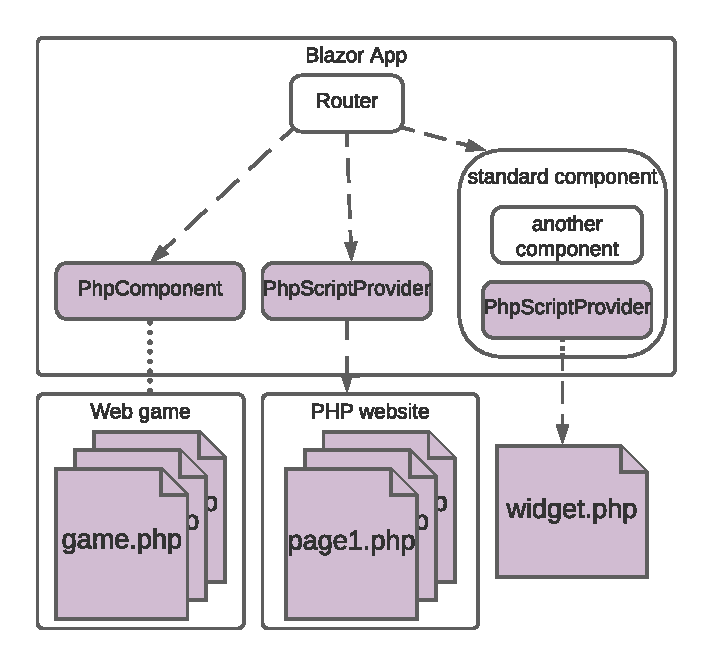
\includegraphics[scale=0.9]{./img/Components}
\caption{Components representing PHP scripts. Arrows represent navigation. 
Dot lines connect a runtime object with the implementation.
}
\label{img12:component}
\end{figure} 
\par
We will focus on the first component, which we will call \texttt{PhpComponent} due to the effort of moving the component concept to PHP.
\texttt{PhpComponent} aims at the third use case.
Despite language differences, we can utilize the common concept of classes and inheritance because Peachpie allows inheriting C\# class in a PHP code.
This feature results in full support of component interface without creating new structures for managing component behavior from PHP.
We can inherit \texttt{ComponentBase} class in PHP and use its methods in the same way as C\# class.
The inheritance offers the required interface in the \textit{WebGame} use case.
At the time of writing, there are also subproblems with the differences of languages.
The current Peachpie version does not support some C\# specifics fully.
The reason can be a hard or impossible representation of C\# entities in PHP.
We should develop some PHP support to enable using the parts of the Blazor interface, which can not be used in PHP directly.
\par
We will call the second type of component \texttt{PhpScriptProvider} expressing an environment for executing standard PHP scripts.
\texttt{PhpScriptProvider} solves the requirements of the remaining use cases \textit{Web}, \textit{OneScript}, and \textit{AllTogether}.
The provider should be able to navigate and execute PHP scripts.
Because the remaining use cases try to hide the integration between PHP and Blazor, the provider should support the following features.
It should pretend a server behavior, which copies everything in the output of PHP script to an HTTP response body rendered by a browser.
Superglobals are often used for obtaining additional information given by the user.
Thus, an ability to fill \texttt{\$\_GET} variable with the URL query part is important.
It should change a standard form functionality, which is sending the form to a server, to save the form information into superglobals, and executing the script again.
We target to load and save files submitted by form transparently in order to provide similar comfort to execute the script on a server side.
A possibility of saving the script context to the next execution is a new opportunity how to keep an application state in PHP script.
We will describe the provider modes.
These modes are intended to solve \textit{Web}, \textit{OneScript}, and \textit{AllTogether} use cases. 
\par
We call the first mode \textbf{Router}, which aims at the \textit{Web} use case, where the implementation is inspired by a github project \squarecite{26}.
It enables to set the provider as a root component.
It handles all navigation events, determines the script name, finds it, and executes the script.
Components defined in PHP code can also be navigation targets.
\par
We call the second mode \textbf{Script}, which aims at the \textit{OneScript} use case.
It enables the provider insertion into a Razor page.
Afterward, the provider executes the specified script.
\par
We call the third mode \textbf{ScriptProvider}, which aims at the \textit{AllTogether} use case.
It enables to navigate the set of scripts with respect to URL.
The navigation is generally maintained by the default \texttt{Router}.
The component only provides navigation to scripts.
\par
These observations lead us to make sure having two different components are rational ways how to separate the problems and offer an understandable difference between the components.


